% -----------------------------------------------------------------------------
\section{Openquake demos}
%
OpenQuake usage help can be obtained by simply typing
\begin{Verbatim}[frame=single, commandchars=\\\{\}, fontsize=\small]
openquake@ubuntu:/media/vbox$ openquake 
\end{Verbatim}
and pressing \texttt{<ENTER>}. The provided info will be 
\begin{Verbatim}[frame=single, commandchars=\\\{\}, fontsize=\small]
usage: openquake [-h] [--version] [--force-inputs] [--config-file CONFIG_FILE]
                 [--output-type {db,xml}]
                 [--log-level {debug,info,warn,error,critical}]
                 [--log-file LOG_FILE] [--list-calculations]
                 [--list-outputs CALCULATION_ID]
                 [--export OUTPUT_ID TARGET_DIR] 
\end{Verbatim}
The main execution of OpenQuake is undertaken via the following 
command-line instruction (note that from this point on we'll indicate the 
the command prompt with a simple \texttt{\$}.

An OpenQuake analysis can be launched with the following command
\begin{Verbatim}[frame=single, commandchars=\\\{\}, fontsize=\small]
$ openquake --\textcolor{red}{config_file}=/PATH/TO/CONFIG/FILE --\textcolor{red}{output_type}=xml
\end{Verbatim}
%
\clearpage
\subsection{I exercise: Peer test Set 1 Test 10}
The first demo we consider, is a simple demo included in the PSHA test 
calculations proposed by \citet{thomas2010}.

The input model consists of a single circular area source as it is 
represented in \ref{fig:demo_peer_set1_test10}; the radius of the source 
is sligthly more than one degree of longitude (at 38 degrees latitude) 
which corresponds to about 88km. 
% ..............................................................................
% . . . . . . . . . . . . . . . . . . . . . . . . . . . . . . . . . . . > Figure
\begin{figure}[htbp]
\begin{center}
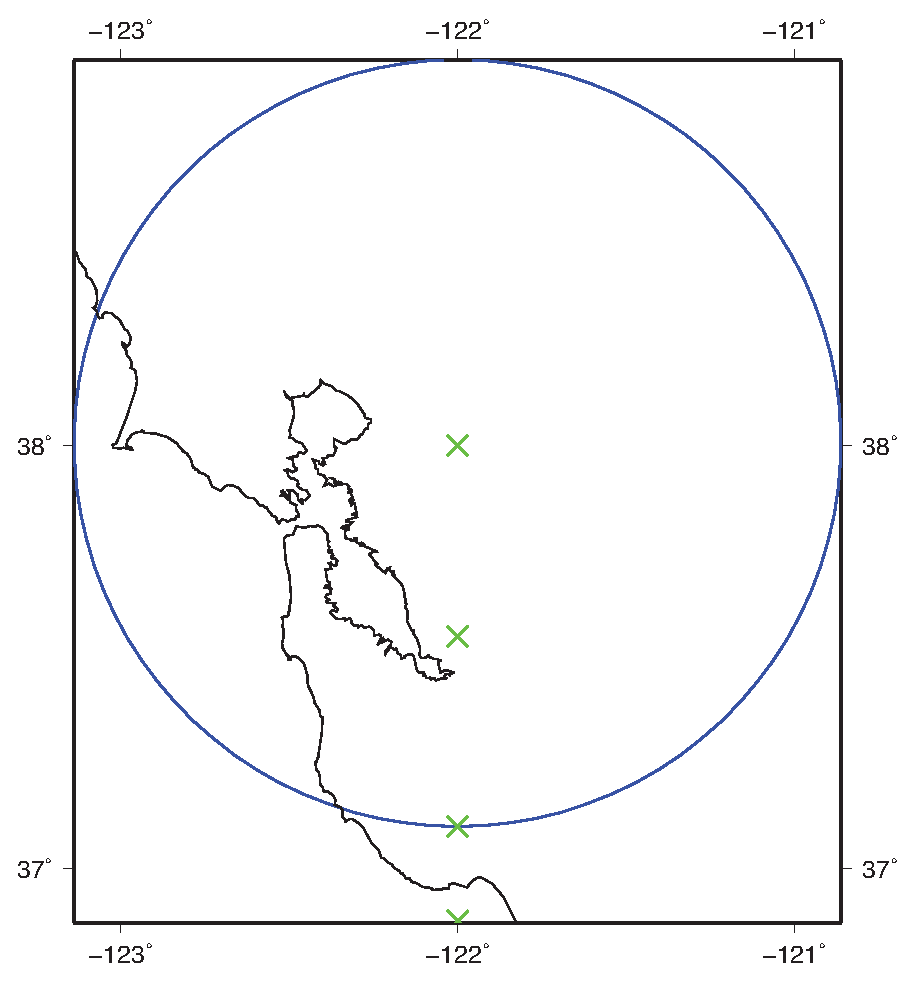
\includegraphics[width=10cm]{./figures/peer_set1_test10/peerSet1test10a.eps}
\caption{PEER Set 1 Test 10: area source geometry and position of sites (green
    crosses)}
\label{fig:demo_peer_set1_test10}
\end{center}
\end{figure}

\clearpage
\subsection{II exercise: Area source demo hazard}
%
The input files for this demos can be found in the folder 
\texttt{area\_source\_demo\_hazard}

The input information consists of a PSHA input model for South East Asia 
developed in the context of the GSHAP project and containing 
\cleardoublepage
